\documentclass[xcolor=pst,dvips,12pt,english,french]{beamer}
\usepackage[backend=biber,style=numeric,firstinits=true, isbn=false, url=false, doi=false, eprint=false]{biblatex}

\bibliography{../biblio3.bib}
\usepackage{graphicx}
\usepackage{babel}
\usepackage[utf8]{inputenc}
\usepackage{lmodern}
\usepackage{beamerthemeshadow}
\usepackage[skip=2pt,font=scriptsize,labelformat=empty]{caption} % Required for specifying captions to tables and figures
\usepackage{pstricks}

\title{Sujet de thèse :}
\author{Fournier Pierre}

\newrobustcmd*{\footlessfullcite}{\AtNextCite{\renewbibmacro{title}{}\renewbibmacro{in:}{}}\footfullcite}


\begin{document}
	\frame{\titlepage} 
	
	\frame{\frametitle{Table of contents}\tableofcontents} 
	
	\section{Contexte}
	
	\subsection{Robotique développementale}
	
	\begin{frame}{La robotique développementale}
		\begin{block}{Un robot peut-il apprendre comme un enfant ?}
			 Comment faire émerger des compétences cognitives avancées de son interaction avec l'environnement ?
		\end{block}
		\begin{columns}
			\begin{column}{0.45\textwidth}
				\begin{exampleblock}{Contraintes}
					\begin{itemize}
						\item \emph{Lifelong learning}
						\item \emph{task-independent architecture}
						\item Complexité croissante des compétences
					\end{itemize}
				\end{exampleblock}
			\end{column}
			\begin{column}{0.45\textwidth}
				\begin{exampleblock}{Inspiration}
					Psychologie développementale, neurosciences, linguistique, biologie évolutionnaire...
				\end{exampleblock}
			\end{column}
		\end{columns}
	\end{frame}
	
	\begin{frame}{Interagir avec un environnement}
		\begin{block}{Embodied, situated robots}
			La cognition émerge chez un organisme par l'interaction avec son environnement, dépendante des capacités sensorimotrices de l'organisme dans cet environnement.
		\end{block}
		\begin{columns}
			\begin{column}{0.55\textwidth}
				\begin{exampleblock}{Autonomous object discovery}
					Interaction avec des objets : 
					\begin{itemize}
						\item Identification
						\item Apprentissage d'affordances
						\item Séquences d'actions
					\end{itemize}
				\end{exampleblock}
			\end{column}
			\begin{column}{0.35\textwidth}
				\vspace{0.5cm}
				\centering
				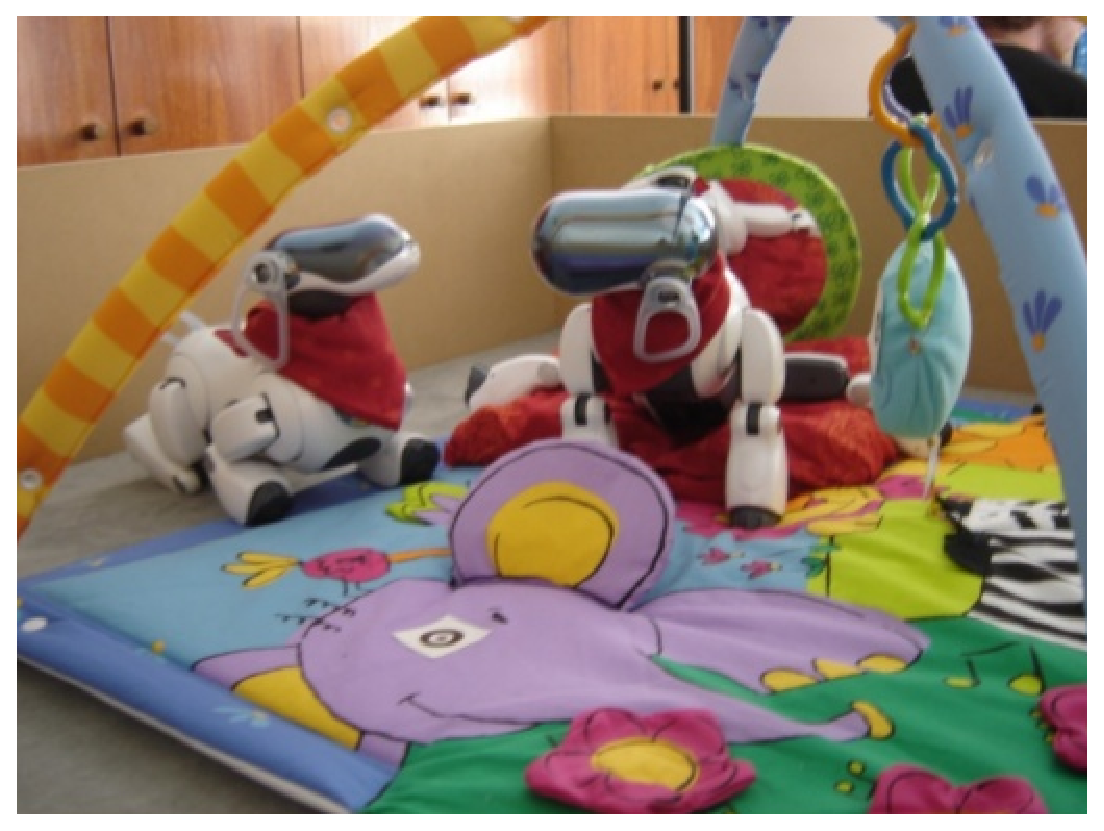
\includegraphics[width=\textwidth]{images/playground.eps}
				\captionof{figure}{The playground experiment}
			\end{column}
		\end{columns}
	\end{frame}
	
	\subsection{Intrinsically motivated reinforcement learning}
	
	\begin{frame}{Quel mécanisme d'apprentissage ?}
		\begin{block}{Apprentissage par renforcement}
			L'agent cherche un comportement décisionnel maximisant les \og récompenses \fg{} fournies par son environnement.
		\end{block}
		\begin{columns}
			\begin{column}{0.45\textwidth}
				\centering
				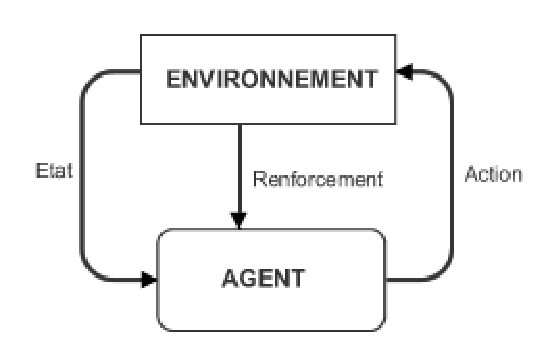
\includegraphics[width=\textwidth]{images/RL1.eps}
			\end{column}
			\begin{column}{0.5\textwidth}
				\begin{exampleblock}{L'origine des récompenses}
					L'environnement lui-même ne fournit que très rarement des \og récompense \fg{} (ex: douleur). 
				\end{exampleblock}
			\end{column}
		\end{columns}
	\end{frame}
	
	\begin{frame}{Motivation intrinsèque}
		\begin{block}{Une récompense interne}
			L'agent définit lui-même et s'attribue des objectifs définissant des récompenses.
		\end{block}
		\begin{columns}
			\begin{column}{0.5\textwidth}
				\begin{exampleblock}{Quelle origine ?}
					\begin{itemize}
						\item \emph{Goal-babbling}
						\item Curiosité artificielle : surprise, compétence, représentation...
					\end{itemize}
				\end{exampleblock}
			\end{column}
			\begin{column}{0.35\textwidth}
				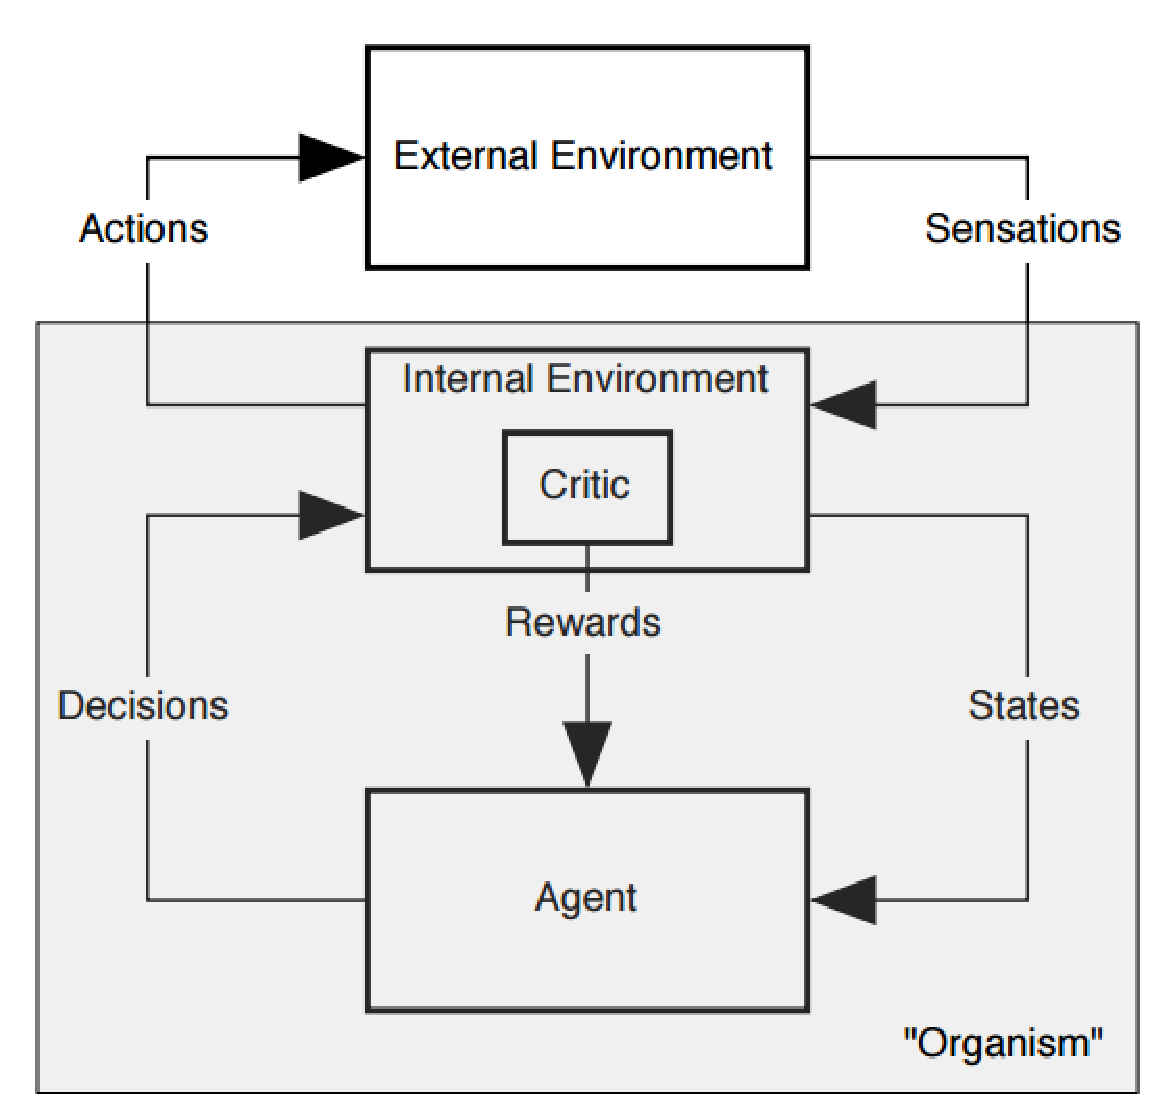
\includegraphics[width=\textwidth]{images/modele_imrl.eps}
			\end{column}
		\end{columns}
	\end{frame}
	
	\section{Positionnement de la thèse}

	\begin{frame}{Positionnement de la thèse}
		\begin{block}{Guidage de l'exploration}
			Au sein d'une tâche de découverte autonome d'un environnement, comment guider et accélérer l'exploration du robot par une interaction avec un tuteur humain ?
		\end{block}
		\begin{exampleblock}{Applications hors apprentissage développemental}
			Personnalisation / amélioration des compétences d'un robot de manière naturelle et sans recourir à la programmation.
			 \\ 
			$\to\,$ Jeu avec un robot de compagnie par exemple.
		\end{exampleblock}
	\end{frame}
	
	\subsection{Interactive reinforcement learning}
	
	\begin{frame}{Interactive reinforcement learning}
		\begin{block}{Principe}
			La récompense provient partiellement d'une interaction en temps réel avec un tuteur (démonstration, guidage,...)
		\end{block}
		\begin{exampleblock}{Labeled to unlabeled guidance}
			L'interprétation de l'interaction n'a pas de raison d'être connue du robot :
			\begin{itemize}
				\item Apprentissage de la tâche 
				\item Apprentissage du sens de l'interaction
			\end{itemize}
		\end{exampleblock}
	\end{frame}
	
	\begin{frame}{Réflexion sur l'interaction}
		\begin{block}{Constat chez les enfants}
			L'interaction elle-même semble être valorisée indépendamment de son objet : aide spontanée, reproduction d'un jeu une fois appris, etc.
		\end{block}
		\begin{exampleblock}{Question}
			En attribuant au sein du mécanisme de motivation intrinsèque une valeur positive à la synchronie entre agent et tuteur, est-il possible de guider l'exploration autonome dans la direction manifestée par les actions du tuteur ? 
		\end{exampleblock}
	\end{frame}
	
	\subsection{Cadre actuel}
	
	\begin{frame}{Cadre de travail actuel}
		\begin{block}{Constat chez les enfants}
			L'interaction elle-même semble être valorisée indépendamment de son objet : aide spontanée, reproduction d'un jeu une fois appris, etc.
		\end{block}
		\begin{exampleblock}{Question}
			En attribuant au sein du mécanisme de motivation intrinsèque une valeur positive à la synchronie entre agent et tuteur, est-il possible de guider l'exploration autonome dans la direction manifestée par les actions du tuteur ? 
		\end{exampleblock}
	\end{frame}

\end{document}